\subsection*{Notação $O$}
    Quando existe um limite assintótico superior, a notacão $O$,é utilizada. Para uma dada função g(n), denotamos por O((g(n)) (lê-se "Ó grande de g de n" ou, "ó de g de n") o conjunto de funções $O(g(n)) =f(n)$( existem constantes positivas $c$ e $n_0$ tais que $0\leq f(n) \leq c*g(n)$ para todo $ n \geq n_0$).
    
Usamos a notação $O$ para dar um limite superior a uma função, dentro de um fator constante. Para todos os valores $n$ em $n_0$ ou à direita de $n_0$, o valor da função $f(n)$ está abaixo de $c*g(n)$.

 Tendo em vista que a notação $O$ descreve um limite superior, quando a empregamos para limitar o tempo de execução do pior caso de um algoritmo temos um limite para o tempo de execução do algoritmo em cada entrada\cite{AlgoritmoCormen2009}.




\subsection{Complexidade O(1)}

A complexidade $O(1)$, ou complexidade de tempo constante, significa que um algoritmo leva o mesmo tempo para executar, independentemente do tamanho da entrada. Isso ocorre porque o algoritmo realiza um número fixo de operações, como calcular a distância entre dois pontos ou acessar um elemento específico em matrizes.

A fim de  demonstrar o sistema de complexidade $O(1)$ será utilizado um exemplo como base, neste exercício  é necessário criar um programa que quantifique diferentes tipos de pisos para uma sala qualquer, onde não basta apenas ter área da sala, pois os pisos se diferem entre inteiros e cortados, então leva-se em consideração os espaços não completos do chão da sala.

A complexidade $O(1)$, trabalha com uma constante durante todo o seu processo, para fins de contagem a constante é desprezada.
Segue o exemplo:
\newpage
\begin{center}
Piso da escola

{ OBI 2018}

Timelimit: $1$	
\end{center}

 O colégio pretende trocar o piso de uma sala de aula e a diretora aproveitou a oportunidade para passar uma tarefa aos alunos. A sala tem o formato de um retângulo de largura $L$ metros e comprimento $C$ metros, onde $L$ e $C$ são números inteiros. A diretora precisa comprar lajotas de cerâmica para cobrir todo o piso da sala. Seria fácil calcular quantas lajotas seriam necessárias se cada lajota fosse um quadrado de $1$ metro de lado. O problema é que a lajota que a diretora quer comprar é um quadrado que possui $1$ metro de diagonal, não de lado. Além disso, ela quer preencher o piso da sala com as diagonais das lajotas alinhadas aos lados da sala, como na figura.

A loja vai fornecer lajotas do tipo $1$: inteiras; do tipo $2$, que correspondem à metade das do tipo $1$, cortadas ao longo da diagonal; e lajotas do tipo $3$, que correspondem à metade do tipo $2$. Veja os três tipos de lajotas na figura.

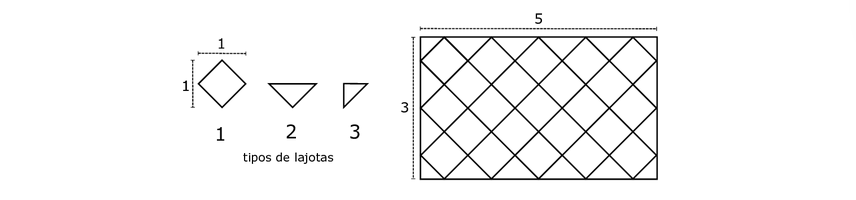
\includegraphics[width=1.0\textwidth]{fig/Piso da Escola.png}
 Está muito claro que sempre serão necessárias $4$ lajotas do tipo $3$ para os cantos da sala. A tarefa que a diretora passou para os alunos é calcular o número de lajotas dos tipos $1$ e $2$ que serão necessárias. Na figura, para $L=3$ e $C=5$, foram necessárias $23$ do tipo $1$ e $12$ do tipo $2$.

Seu programa precisa computar, dados os valores de $L$ e $C$, a quantidade de lajotas do tipo $1$ e do tipo $2$ necessárias.

\vspace{0.3cm}
\textbf{Entrada}

A entrada consiste de um único número inteiro $L$ indicando a largura da sala. A segunda linha contém um inteiro $C$ representando o comprimento da sala, conforme dados da tabela~\ref{tabela01}. 

\vspace{0.3cm}
\textbf{Saída}

Imprima duas linhas na saída. A primeira deve conter um inteiro, representando o número de lajotas do tipo $1$ necessárias. A segunda deve conter um inteiro, indicando o número de lajotas do tipo $2$.

\textbf{Restrições}
\begin{itemize}
    \item $1 \leq L,C \leq 100$
\end{itemize}

\begin{table}[!ht]
    \centering
    \begin{tabular}{|p{7cm}|p{7cm}|}
        \hline
        \begin{center}
            \vspace{-0.3cm}
            \textbf{Exemplos de Entrada}
            \vspace{-0.3cm}
        \end{center} 
         &  
        \begin{center}
            \vspace{-0.3cm}
            \textbf{Exemplos de Saída}
            \vspace{-0.3cm}
        \end{center} \\ \hline
         \texttt{3} & \texttt{23} \\
         \texttt{5} & \texttt{12} \\
         \hline
         \texttt{1} & \texttt{1} \\
         \texttt{1} & \texttt{0}\\
         \hline
    \end{tabular}
    \caption{Exemplos de entradas e saídas}
    \label{tabela01}
\end{table}

%---------------------------------------------


\begin{table}[ht]
\centering

\label{tab:algoritmo1}
\begin{tabular}{|p{8cm}|c|c|}
\hline
\textbf{\cellcolor[HTML]{C0C0C0}Algoritmo} & \textbf{\cellcolor[HTML]{C0C0C0}Custo} & \textbf{\cellcolor[HTML]{C0C0C0}Complexidade} \\
\hline
\begin{minipage}{8cm}
{
        \begin{algorithm}[H]
            \caption{Piso da Sala}
            \label{alg:01}
            \SetAlgoLined
          \small  \Inicio{
            \textit{Declare} $L, C, T1, T2$ \textit{inteiro} \\
                \textit{Leia} $T1, T2$ \\
                $T1 \leftarrow L * C + ( L - 1) * ( C - 1)$ \\
                $T2 \leftarrow ( L - 1) * 2 + ( C - 1) * 2$ \\
                \textit{Escreva} $T1$ \\
                \textit{Escreva} $T2$ \\
                }
        \end{algorithm}}
\end{minipage} 
& 
\begin{minipage}{2cm}

C1 \\
C2\\
C3 \\
C4 \\
C5 \\
C6 \\
C7 \\
C8 \\
K\\
\end{minipage}
&
\begin{minipage}{2cm}

O(1) \\
O(1) \\
O(1) \\
O(1) \\
O(1)\\
O(1)\\
O(1) \\
O(1) \\
O(1)\\

\end{minipage}
\\
\hline
\end{tabular}
\end{table}


\begin{equation}
T(n)=({C_1}*1)+({C_2}*1)+({C_3}*1)+({C_4}*1)+({C_5}*1)+({C_6}*1)+({C_7}*1)+({C_8}*1)
\end{equation}

\begin{equation}T(n)=({C_1}+{C_2}+{C_3}+{C_4}+{C_5}+{C_6}+{C_7}+{C_8})*1\end{equation}
\begin{equation}\textit{Considere K} = {C_1}+{C_2}+{C_3}+{C_4}+{C_5}+{C_6}+{C_7}+{C_8}\end{equation}

\begin{equation}
    T(n)= K*1 = O(1)
\end{equation}
\begin{center}
\begin{minipage}{0.5\textwidth}
    \lstinputlisting[language=C++]{code/piso1.cpp}
\end{minipage}
\end{center}
\newpage